\documentclass{article}

\usepackage[utf8]{inputenc}
\usepackage{graphicx}


\usepackage[french]{babel}


\title{L'épopée projet 2}
\author{Edwige Cyffers \and Maxime Darrin}
\date{}


\begin{document}

\maketitle
\tableofcontents

\newpage

\section{Les origines du mal}

	Au commencement était un Tetris.
	
	\paragraph{}
	Un peu buggé, certes. Mais issu d'une belle expérience. Oui, on pouvait partir de rien, avancer petit à petit, et finir par transformer quelques litres de thé en un Tétris avec son et couleurs. Avec cette première expérience est née une certitude : ensemble, nous pouvions aller bien plus loin que chacun de notre côté. Bref, nous formions un vrai binôme.
	
	Parce que c'était lui, parce que c'était moi.		
	Parce qu'elle était elle, parce j'étais moi.
	
	Alors nous avons récidivé. Nous nous sommes remis à l'ouvrage. Emportés par notre élan, nous avons fait plus que ce que nous devions faire. Catégorisés en intermédiaire (parce que nous avions fait du CamlLight en prépa, et rien de plus pour Edwige), nous avons pourtant fait tout ce qui était demandé aux avancés.	
	
	\paragraph{}
	Dès lors, le mal était fait, l'engrenage s'était enclenché, nous allions continuer ce rythme effréné jusqu'à la fin de projet 2
	
	De toute façon, il ne faut pas faire de projet si on veut avoir des weekend.
	
	%~\ref{s:orga}

\section{La lutte}

	
%\label{s:orga}
	L'interpréteur s'est peu à peu construit. Malgré un léger désaccord initial sur l'implémentation des fonctions, nous avons sorti du néant un code, parfois lourd, parfois maladroit, mais qui faisait ce qu'on lui demandait.
	
	Heureusement, de valeureux relecteurs \footnote{Parfois appelés correcteurs, et plus exactement Henning Basold,
	Daniel Hirschkoff et 
	Bertrand Simon} veillaient au grain.

	\subsection{Quelques motifs récurrents}
	
		Ce combat a donc été marqué par un certain nombre de techniques de travail plus ou moins évoluées
		
		\begin{itemize}
			\item La méthode de la lecture de parseur.out
			\item La méthode de la dichotomie pour trouver l'erreur en temps  du problème à coup de commentaires biens choisis
			\item La méthode exponentielle : lorsqu'on est convaincu que le résultat est proche, il suffit de faire un parcours exhaustif de toutes les possibilités
			\item La méthode de la réécriture complète : simple et définitive
			\item La méthode de finalement c'est juste un bonus, parfois appelée méthode du renoncement par manque de temps\footnote{Qui, il faut bien l'avouer, nous brise le cœur.}
			\item La méthode de "il semblerait que ça marche" : hélas, n'arrive pas souvent.
		\end{itemize}
	
	\subsection{Commits en tout genre}
	
		Ces méthodes de travail ont pu transparaître dans le noms de certains commits, dont nous avons donc gardé un petit florilège.
		
		\begin{figure}[h]
			\centering		
		\begin{tabular}{l|l|c}
			Date & Auteur & Nom\\
			
			10/05/2018 & Edwige & toujours pas de let, mais la confirmation que ce qui marche marche \\
			08/05/2018 & Edwige & magnifiques exceptions, je vais pouvoir en rêver cette nuit \\
			04/05/2018 & Maxime & Yolo jsuis le meilleur \\
			04/05/2018 & Maxime & following the consignes: -outcode \\
			04/05/2018 & Maxime & exception consigne friendly \\
			03/05/2018 & Maxime & jsuis un peu nul parfois \\
			02/05/2018 & Edwige & je suis contente \\
			02/05/2018 & Edwige & en gros les fonctions,il faut que je trouve où est l'erreur \\
			01/05/2018 & Edwige & petit mélange de type, galimatia à reprendre à tête reposée \\
			24/04/2018 & Maxime & Woualleeez \\
			24/04/2018 & Edwige & ok \\
			23/04/2018 & Edwige & j'ai viré le news pour un minimum de cohérence \\
			22/04/2018 & Maxime & je crois que j'ai fait un truc qui marche presque \\
			21/04/2018 & Maxime & bricolage du matin \\
			21/04/2018 & Maxime & debut du rangement \\
			20/04/2018 & Maxime & J'ai bricolé, ça a marché: cf exception\_4.ml \\
			18/04/2018 & Maxime & LOL CA MARCHE WTF \\
			18/04/2018 & Edwige & un jour ça marchera peut-être, j'y reviens quand mon cerveau remarche \\
			18/04/2018 & Edwige & quand sur un malentendu ça compile \\
			18/04/2018 & Edwige & un nouveau constructeur pour toujours plus de clarté \\
			18/04/2018 & Edwige & un début moins faux \\
			18/04/2018 & Edwige & début des ontinuations, début des problèmes \\			
		\end{tabular}
	\caption{Best Of des meilleurs commits}
\end{figure}


	\section{Inutile}
	\subsection{Following the consignes}
	Parce que c'est demandé, nous le mettons discrètement \cite{Landin:1966:NPL:365230.365257}. Parce que ce n'est pas demandé, mais que ça semble plus que nécessaire : 
	
	\subsection{Fouine}
	La fouine (Martes foina) est une espèce de mammifères carnivores d'Europe et d'Asie, au pelage gris-brun, courte sur patte et de mœurs nocturnes. C'est une martre (ou marte) faisant partie de la famille des Mustélidés, au même titre que la belette, le blaireau, la loutre, le putois ou le furet, petits mammifères carnivores se caractérisant souvent par leur odeur forte.\cite{wiki:Fouine}
	
	\begin{figure}[h]
		\centering
		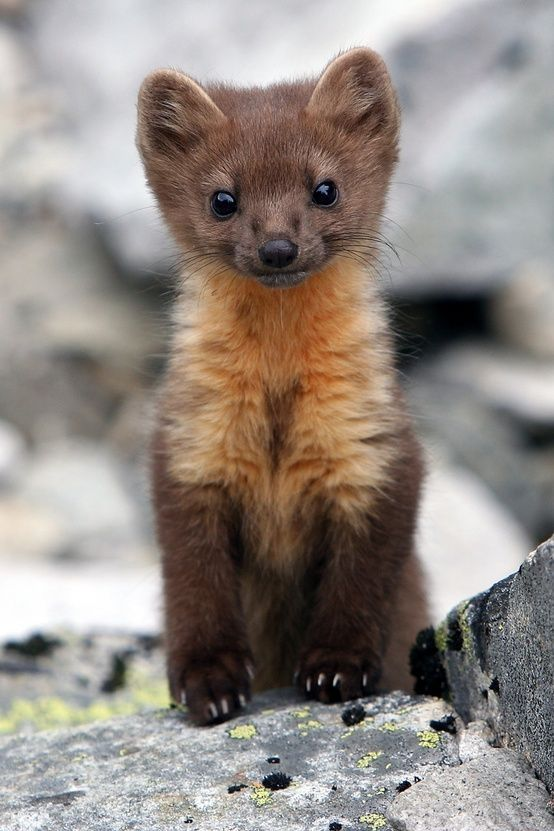
\includegraphics[scale=0.3]{img/fouine}
		\caption{Une fouine}
	\end{figure}
	
	\section{Notre Fouine}
	
	\subsection{Documentation}
	
	La documentation de notre interpreter se trouve dans le dossier \emph{doc/} après la compilation du projet. Un readme à propos de l'ensemble du projet est présenté dans le dossier rapport. Et un Readme concernant uniquement le rendu 4 est à la racine du projet.
	
	\subsection{Spécifications originelles}
	
	On peut trouver la spécification du langage fouine sur le site internet du département d'informatique de l'ENS de Lyon\cite{di:fouine}.
	
	\subsection{Bonus}
	
	Nous avons implémenté les bonus suivants, et nous avons essayé de les maintenir malgré la difficulté croissante du sujet. De plus nous proposons une documentation de notre projet utilisant ocamldoc. Celle-ci est générée automatiquement en effectuant un make ou un make doc dans le dossier src.
	
	\begin{itemize}
		\item n-uplets (avec une limitation syntaxique: on impose des parenthèses autours systématiquement)
		\item Les type sommes (même limitation)
		\item Le pattern Matching (uniquement le match ... with et sans les when)
		\item Les listes
		\item L'inférence de type
	\end{itemize}



\section{Projet intégré, à nous deux maintenant}
	
	Elle ne savait pas ce qu'était un parseur, il ne savait pas utiliser de fonctionnelles. Et pourtant, avec un peu de chance, beaucoup de travail, de temps, de détermination, et surtout avec une collaboration sans faille, nous avons fait quelque chose dont nous sommes fiers. 
	
	Et un projet de plus ensemble. Nous attendons le prochain de pied ferme.
	
\section{Remerciements}
\subsection{A nos amis \& amours}
Nous souhaitons tout d'abord nous remercier l'un l'autre pour tout le travail accompli, le soutien sans faille et la patience infinie nécessaires pour supporter l'autre\footnote{Spoiler: Cela a probablement été plus dur pour l'une que pour l'autre, qui l'en remercie} tout au long du projet. 

Nous remercions aussi dans cet ordre nos moitiés respectives\footnote{Eléonore et Lucas} pour leur compréhension pour les nuits passées en binôme plutôt qu'en couple; le groupe d'Antonin et Alain avec qui nous avons parfois, voire souvent, unis nos forces; mais aussi nos fidèles compagnons de route: Câlin et Totoro qui ont permis un débuggage efficace du code sans appeler à l'aide.
\subsection{A nos encadrants}
Finalement et plus sérieusement, nous tenons à signifier aux encadrant de Projet 2 que nous avons noté, et apprécié, les efforts de bienveillance et d'organisation du projet pour le rendre accessible à toutes et tous, quel que fût le niveau de caml initial. Nous avons été d'autant plus sensibles à ces efforts qu'ils ne sont malheureusement pas faits dans d'autres cours.


\bibliographystyle{plain}
\bibliography{biblio}

\end{document}
